\documentclass{standalone}
\usepackage{tikz}
\usepackage{pgfplots}

\pgfplotsset{width=20cm,compat=1.5}

\begin{document}

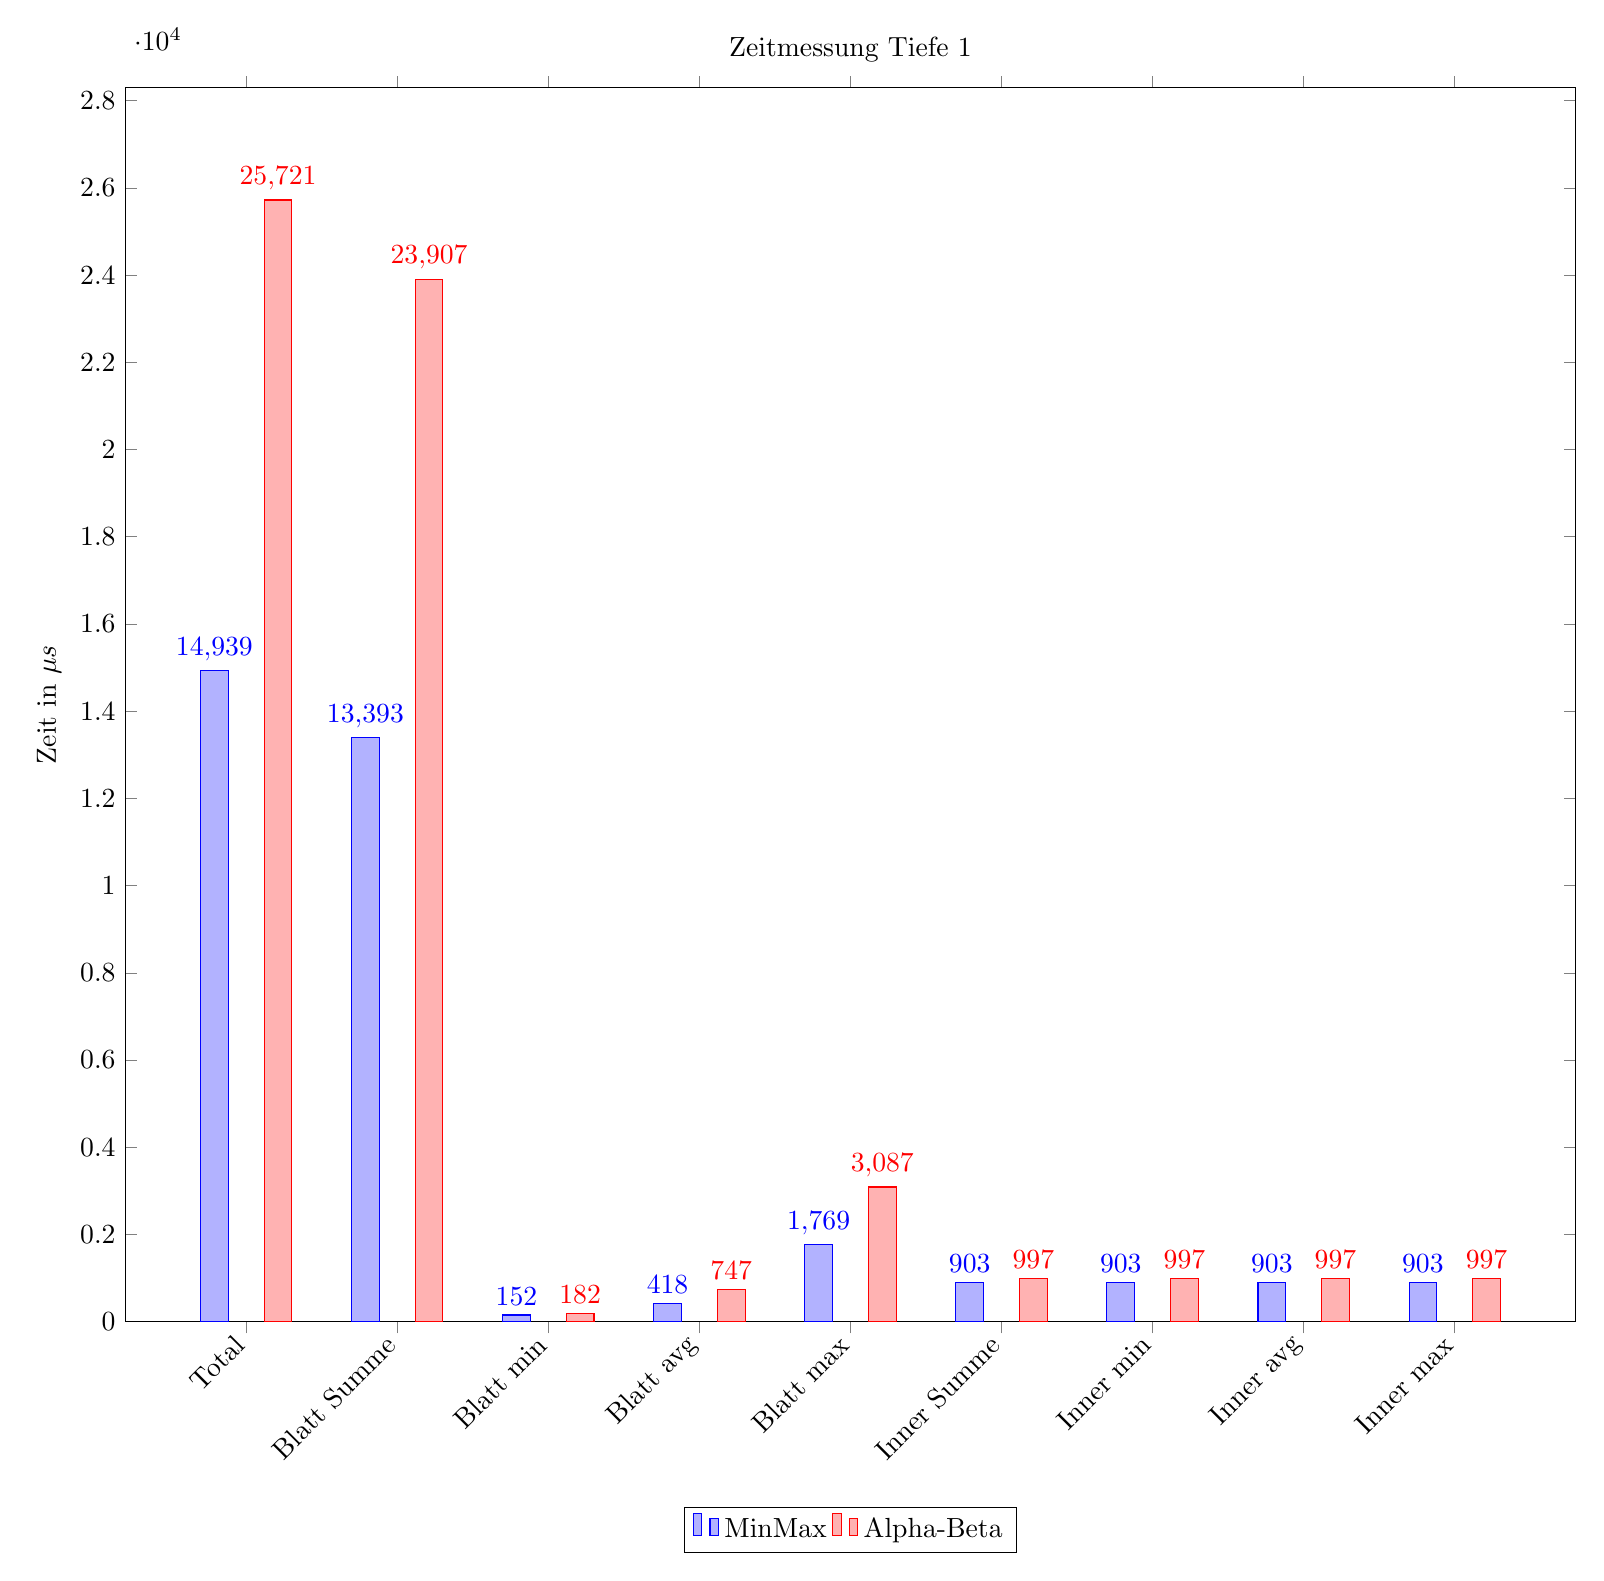
\begin{tikzpicture}
  \begin{axis}[
    title=Zeitmessung Tiefe 1,
    ybar=13pt,
    legend style={at={(0.5,-0.15)},
    anchor=north,
    legend columns=-1},
    ylabel={Zeit in $\mu s$},
    ymin = 0,
    symbolic x coords={
      Total,
      Blatt Summe,
      Blatt min,
      Blatt avg,
      Blatt max,
      Inner Summe,
      Inner min,
      Inner avg,
      Inner max
    },
    xtick=data,
    nodes near coords,
    nodes near coords align={vertical},
    x tick label style={rotate=45,anchor=east}
  ]
    \addplot coordinates{
      (Total,       14939)
      (Blatt Summe, 13393)
      (Blatt min,     152)
      (Blatt avg,     418)
      (Blatt max,    1769)
      (Inner Summe,   903)
      (Inner min,     903)
      (Inner avg,     903)
      (Inner max,     903)
    };
    \addplot coordinates{
      (Total,       25721)
      (Blatt Summe, 23907)
      (Blatt min,     182)
      (Blatt avg,     747)
      (Blatt max,    3087)
      (Inner Summe,   997)
      (Inner min,     997)
      (Inner avg,     997)
      (Inner max,     997)
    };
    \legend{
      MinMax,
      Alpha-Beta
    }
  \end{axis}
\end{tikzpicture}


\end{document}